\documentclass[12pt]{article}

\usepackage{fullpage}
\usepackage{multicol,multirow}
\usepackage{tabularx}
\usepackage{ulem}
\usepackage[utf8]{inputenc}
\usepackage[russian]{babel}
\usepackage{graphicx}
\usepackage{indentfirst}


\begin{document}

\section*{Лабораторная работа №\,6 по курсу дискрeтного анализа: Длинная арифметика}

Выполнил студент группы М8О-207Б МАИ \textit{Цапков Александр}.

\subsection*{Условие}

\begin{enumerate}
\item Необходимо разработать программную библиотеку на языке С или С++, реализующую простейшие арифметические действия и проверку условий над целыми неотрицательными числами. На основании этой библиотеки нужно составить программу, выполняющую вычисления над парами десятичных чисел и выводящую результат на стандартный файл вывода.

Список арифметических операций:

Сложение (+).

Вычитание (-).

Умножение (*).

Возведение в степень (\^).

Деление (/).

В случае возникновения переполнения в результате вычислений, попытки вычесть из меньшего числа большее, деления на ноль или возведении нуля в нулевую степень, программа должна вывести на экран строку Error.

Список условий:

Больше (>).

Меньше (<).

Равно (=).

В случае выполнения условия программа должна вывести на экран строку true, в противном случае — false.

Количество десятичных разрядов целых чисел не превышает 100000. Основание выбранной системы счисления для внутреннего представления «длинных» чисел должно быть не меньше 10000.
\item Вариант: 1
\end{enumerate}

\subsection*{Метод решения}
Длинная арифметика — это набор программных средств (структуры данных и алгоритмы), которые позволяют работать с числами гораздо больших величин, чем это позволяют стандартные типы данных.

Основная идея заключается в том, что число хранится в виде массива его цифр.
Цифры могут использоваться из той или иной системы счисления, в данной ЛР применяются десятичная система счисления и её степени: десять тысяч, миллиард (я использкую миллиард)

Операции над числами в этом виде длинной арифметики производятся с помощью "школьных" алгоритмов сложения, вычитания, умножения, деления столбиком. В данной описана работа только с неотрицательными длинными числами.


Источники: https://e-maxx.ru/

\subsection*{Описание программы}

Моя программа состоит из 2-х файлов: LongArifm.hpp с реализацией длинной арифметики и основного файла программы main.cpp. В файле LongArifm.hpp написан класс длинной арифметики с почти всеми перегружинными операциями над числами, а также вводом и выводом (cin и cout). В privat находится только vector разрядов и метод size. все пергруженные операции, а также методы swap и shift реализованы в public. Тип данных для разряда - int, но во многих функциях встречается $ull$, так как при перемножении $10^9$ на $10^9$ получившиеся число не влезает в $int$.

\subsection*{Дневник отладки}

1-я посылка: неправильный ответ, ошибка в делении на маленькое число.

2-я посылка: time limit, увеличил разряд.
 
3-5 посылка: неправильный ответ, ошибка была в неприведении типов в функции степени, когда число выходило за int.

6-я посылка: ожидает подтверждения.

\subsection*{Тест производительности}
Основной интерес представляет функуия деления, осимптотика которой не так очивидна, но на графике можно заметить, что она линейна.

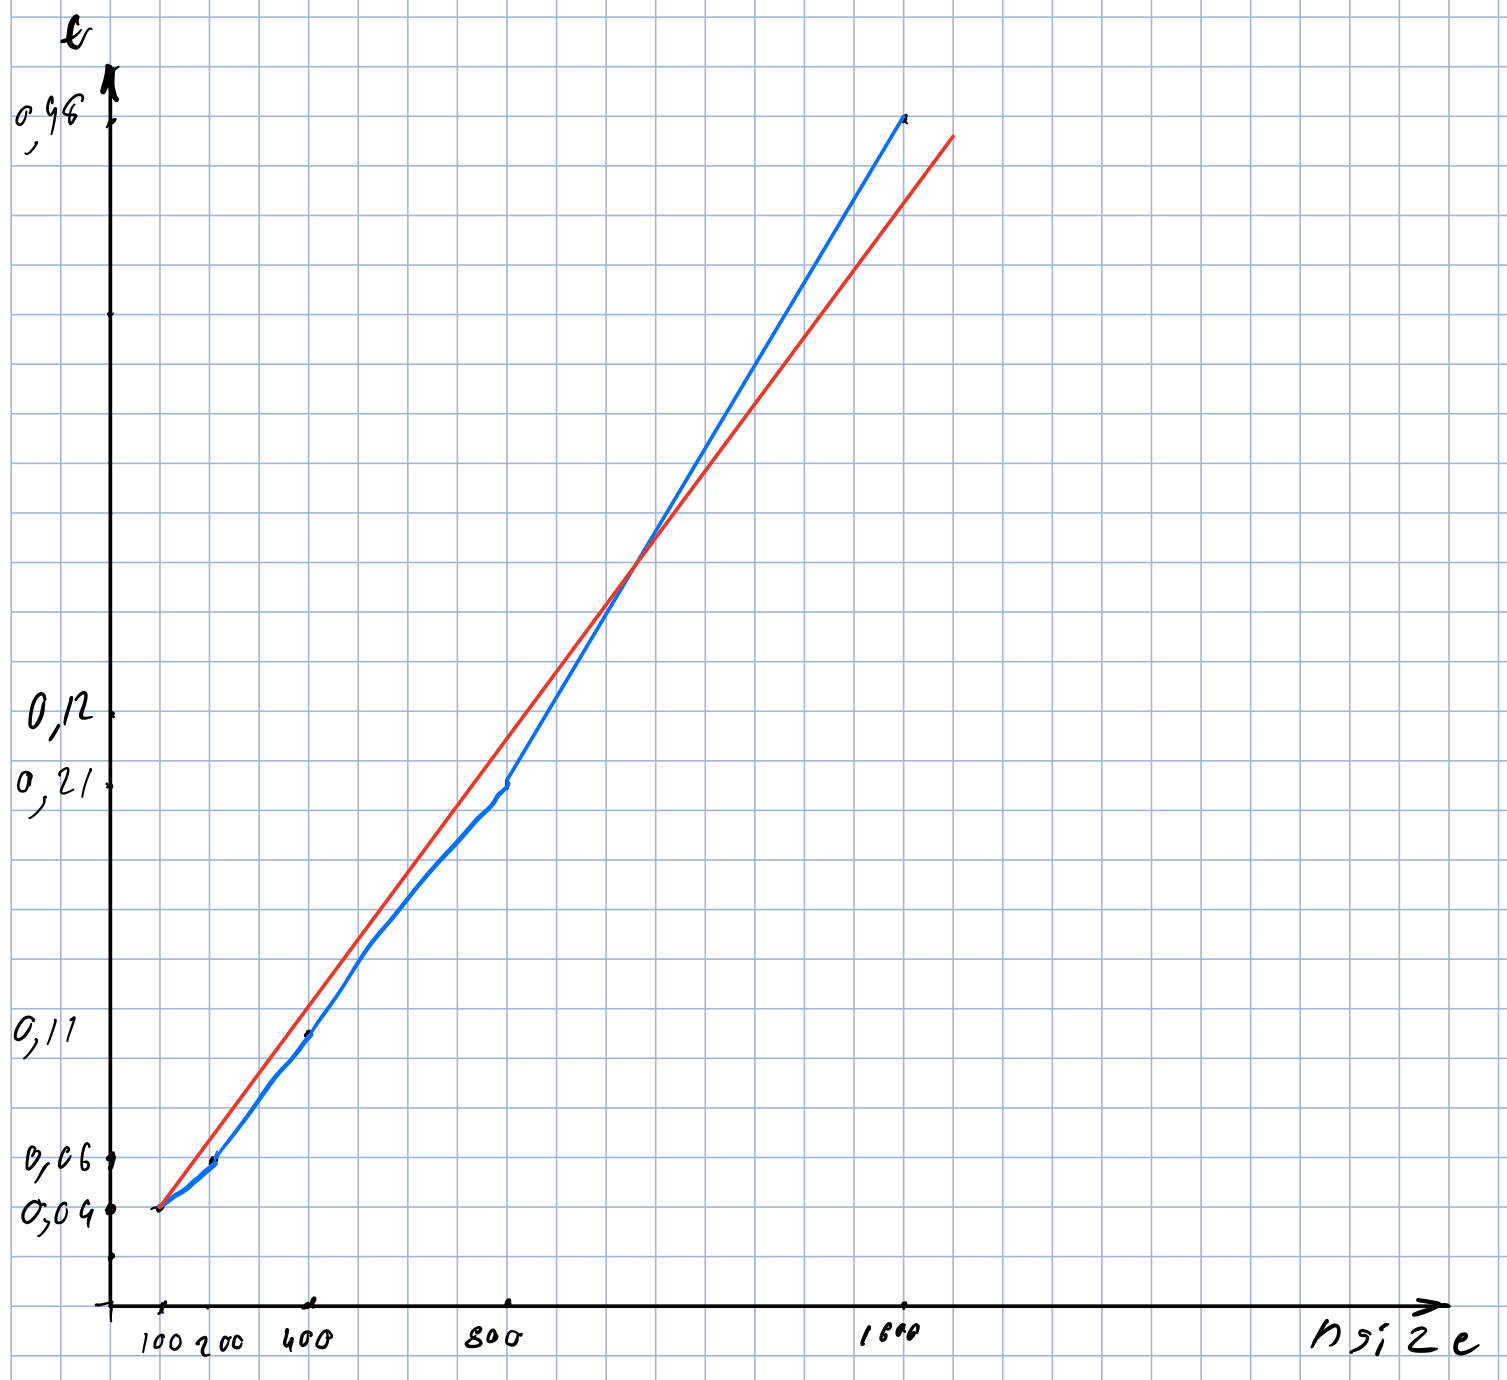
\includegraphics[width=\linewidth]{6.png}

\subsection*{Выводы}

В данной ЛР мне пришлось познакомитться с длинной арифметикой. Интересно реализовавать то чем достаточно часто пользуешься, но не задумываешься об этом (Больние числа питона). Я мог бы использовать свою собственную библиотеку в дальнейшем, но я планирую ее дороботать. К примеру для перемножения больших чисел можно использовать алгоритм Карацубы, который имеет асимпотику меньше квадратичной.

\end{document}

